% ------------------------------------------------------------------------
% ------------------------------------------------------------------------
% Modelo de trabalho acadêmico (Dissertações e Teses) do Programa de Pós-
% graduação em Física da Universidade Federal de Minas Gerais.
% Esse modelo é baseado na classe abntex2 (http://www.abntex.net.br)
% 
% ------------------------------------------------------------------------
% ------------------------------------------------------------------------

\documentclass[
	% -- opções da classe memoir --
	12pt,				% tamanho da fonte
	openright,			% capítulos começam em pág ímpar (insere página vazia caso preciso)
	twoside,			% para impressão em frente e verso. Oposto a oneside ---- Este comando ajusta automaticamente as margens
	a4paper,			% tamanho do papel. 
	english,			% idioma adicional para hifenização
%	french,				% idioma adicional para hifenização basta retirar o comentário para utilizar
%	spanish,			% idioma adicional para hifenização basta retirar o comentário para utilizar
	brazil				% o último idioma é o principal do documento
	]{abntex2}

% ---
% Pacotes básicos 
% ---
\usepackage{lmodern}			% Usa a fonte Latin Modern			
\usepackage[T1]{fontenc}			% Selecao de codigos de fonte.
\usepackage[utf8]{inputenc}		% Codificacao do documento (conversão automática dos acentos)
\usepackage{indentfirst}			% Indenta o primeiro parágrafo de cada seção.
\usepackage{color}				% Controle das cores
\usepackage{graphicx}			% Inclusão de gráficos
\usepackage{microtype} 			% para melhorias de justificação
\usepackage{relsize}				% usado para definir tamanho de fontes no sumário
% ---

% ---
% Pacotes úteis 
% ---
\usepackage[final]{pdfpages}		% Para incluir arquivos pdf externos
\usepackage{amsmath,amssymb,amsthm}	% Pacote para melhorar apresentação de fórmulas matemáticas, símbolos e teoremas, respectivamente	
\usepackage{pdflscape} 		% Pacote para adicionar páginas em formato paisagem
\usepackage{multirow}			% Permite criar céluas com várias colunas ou linhas em tabelas
\usepackage{adjustbox}			% Pacote para ajustar a largura e altura de objetos como tabelas
%\usepackage{imakeidx}			% Gera o índice
% ---

\usepackage{lipsum}	 % pacote usado para gerar os textos dos apêndices e anexos

% ---
% Pacotes de citações
% ---
\usepackage[brazilian,hyperpageref]{backref}	 % Inclui um link nas referências para a página onde o documento foi citado.
\usepackage{cite}
\usepackage[fixlanguage]{babelbib}
\selectbiblanguage{brazil}


% --- 
% CONFIGURAÇÕES DE PACOTES
% --- 

% ---
% Configurações do pacote backref
% Usado sem a opção hyperpageref de backref
\renewcommand{\backrefpagesname}{Citado na(s) página(s):~}
% Texto padrão antes do número das páginas
\renewcommand{\backref}{}
% Define os textos da citação
\renewcommand*{\backrefalt}[4]{
	\ifcase #1 %
		Nenhuma citação no texto.%
	\or
		Citado na página #2.%
	\else
		Citado #1 vezes nas páginas #2.%
	\fi}%
% ---

% ---
% Informações de dados para CAPA e FOLHA DE ROSTO
% ---
\titulo{Synchronization of Phase Oscilators}
\autor{Kevin Liu Rodrigues}
\local{Belo Horizonte}
\data{2020}
\orientador{Ronald Dickman}
\coorientador{Kevin Wood}
\tipotrabalho{Tese (Doutorado)}
\preambulo{Tese apresentada ao Programa de Pós-Graduação em Física do Instituto de Ciências Exatas da Universidade Federal de Minas
Gerais como requisito parcial para obtenção do título de Doutor em Ciências.}


% ---
% Configurações de aparência do PDF final
% ---
% alterando o aspecto da cor azul
\definecolor{blue}{RGB}{41,5,195}

% informações do PDF
\makeatletter
\hypersetup{
     	%pagebackref=true,
		pdftitle={\@title}, 
		pdfauthor={\@author},
    	pdfsubject={\imprimirpreambulo},
	    pdfcreator={LaTeX with abnTeX2},
		pdfkeywords={abnt}{latex}{abntex}{abntex2}{trabalho acadêmico}, 
		colorlinks=false,       		% false: boxed links; true: colored links
    	linkcolor=blue,          	% color of internal links
    	citecolor=blue,        		% color of links to bibliography
    	filecolor=magenta,      		% color of file links
		urlcolor=blue,
		bookmarksdepth=4
}
\makeatother
% --- 

% --- 
% Espaçamentos entre linhas e parágrafos 
% --- 

% O tamanho do parágrafo é dado por:
\setlength{\parindent}{1.3cm}

% Controle do espaçamento entre um parágrafo e outro:
\setlength{\parskip}{0.2cm}  % tente também \onelineskip

% ---
% compila o indice, caso haja.
% ---
%\makeindex
% ---

% ----
% Início do documento
% ----
\begin{document}

% Seleciona o idioma do documento (conforme pacotes do babel)
\selectlanguage{english}
%\selectlanguage{brazil}

% Retira espaço extra obsoleto entre as frases.
\frenchspacing 

% ----------------------------------------------------------
% ELEMENTOS PRÉ-TEXTUAIS
% ----------------------------------------------------------
\pretextual


% ---
% Folha de rosto
% (o * indica que haverá a ficha bibliográfica e deverá ser usado para teses 
%   e dissertações. Para projetos, favor retirar o *)
% ---
\imprimirfolhaderosto*
% ---

% ---
% Inserir a ficha bibliografica
% ---

%  A ficha catalografica, preparada pela biblioteca do departamento de física da UFMG é
% um elemento obrigatório para teses e dissertações. Inclua o arquivo pdf fornecido de acordo
% com o comando abaixo, modificando o nome e a localização do arquivo quando necessário.
%
\begin{fichacatalografica}
    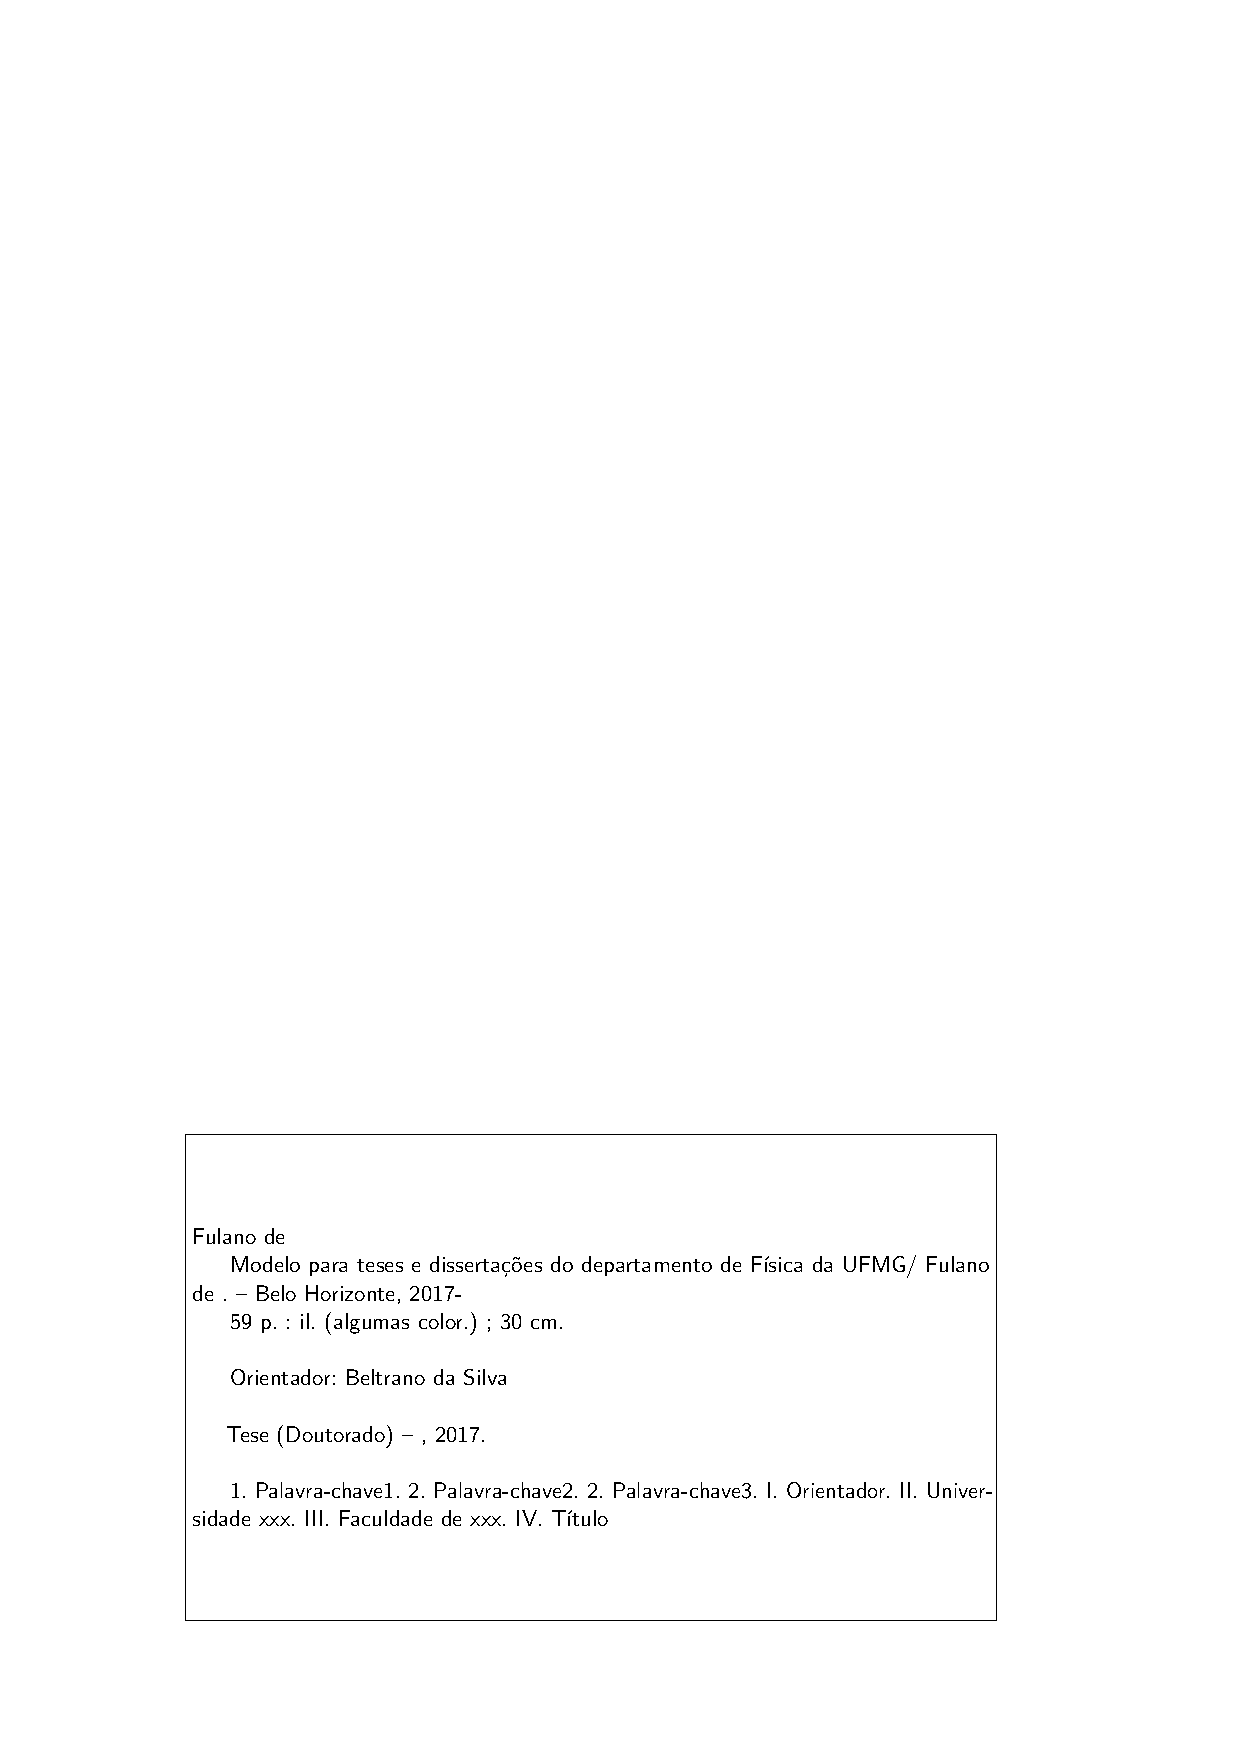
\includepdf{fig/ficha-catalografica.pdf}
\end{fichacatalografica}

% ---
% Inserir folha de aprovação
% ---

% A folha de aprovação é um elemento obrigatório da versão final do trabalho e deverá ser incluído
% conforme comando abaixo.
%
% TODO: na versao final incluir a ficha de aprovacao
\begin{folhadeaprovacao}
     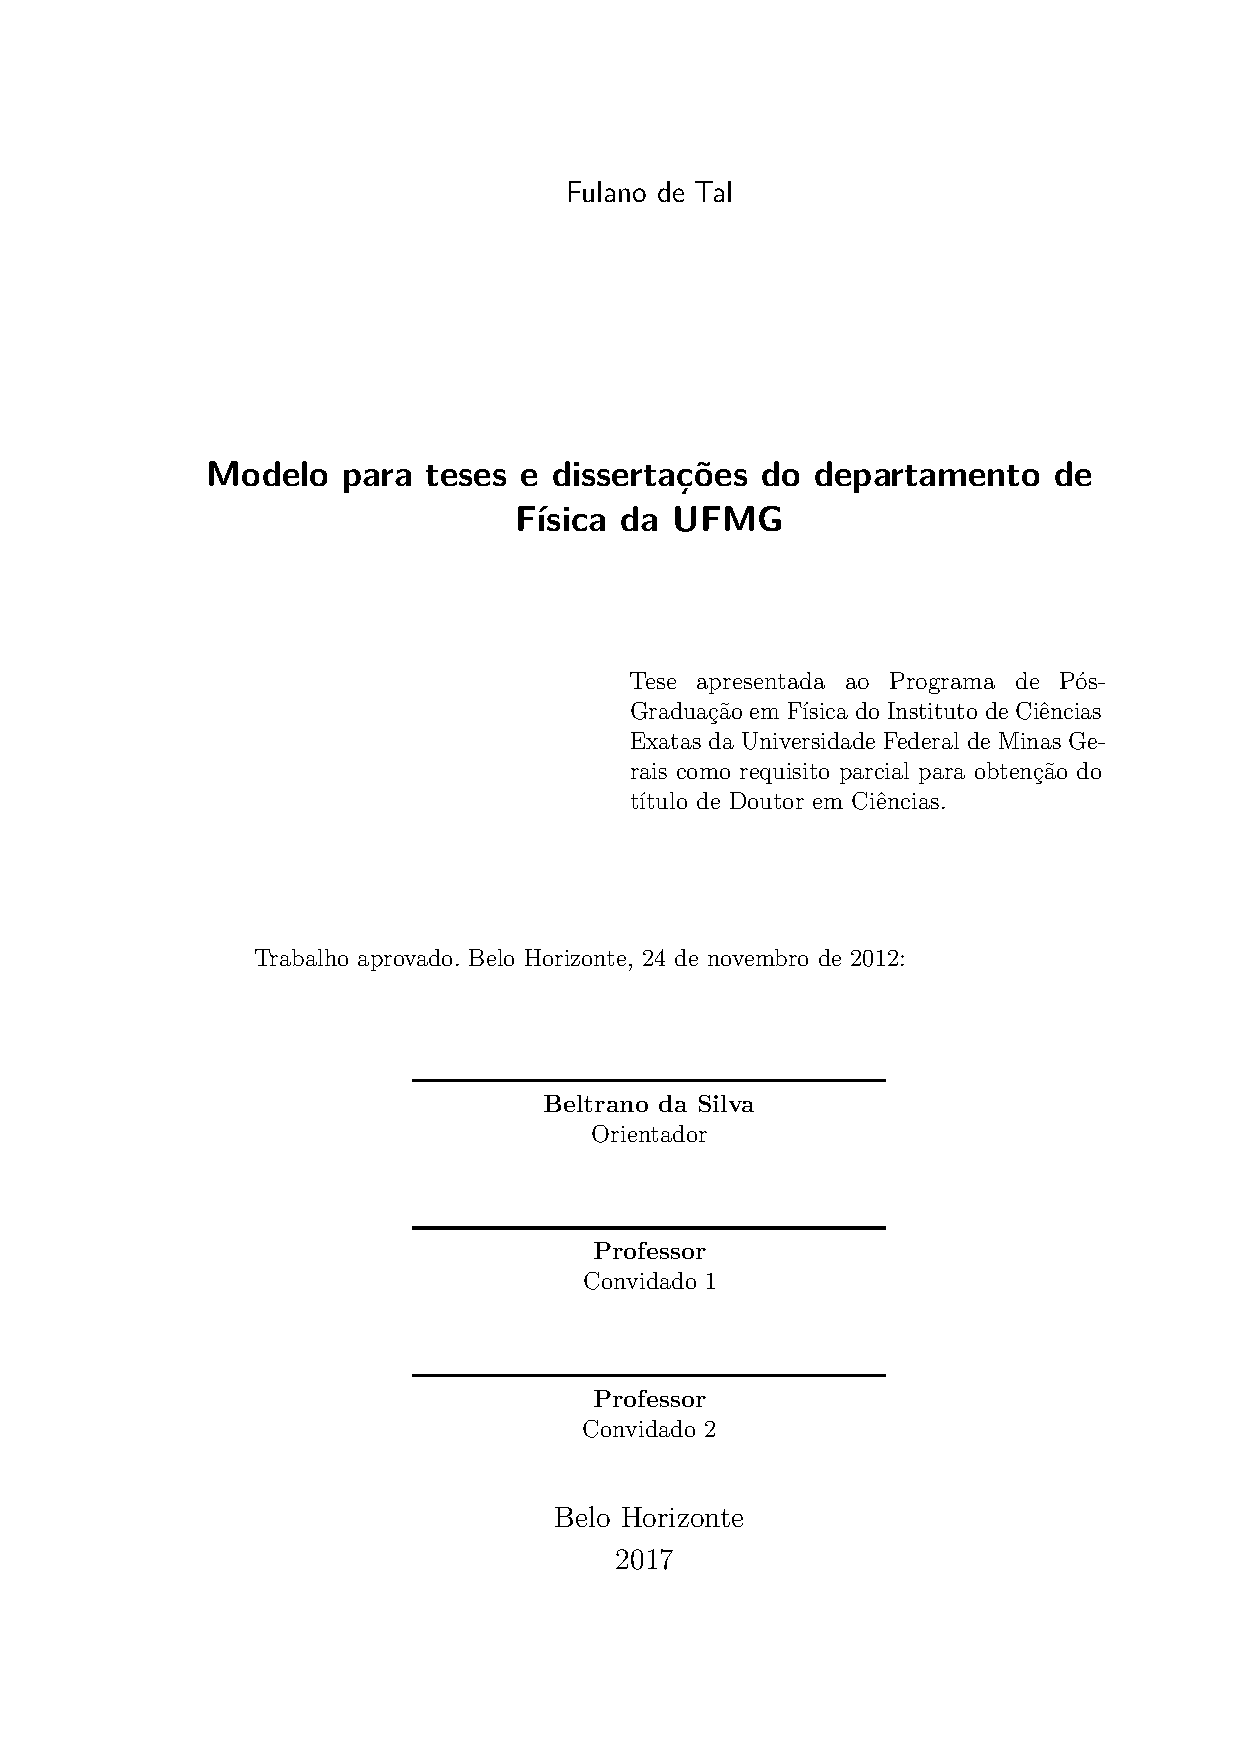
\includepdf{fig/folhadeaprovacao.pdf}
\end{folhadeaprovacao}
%


% ---
% Dedicatória - OPCIONAL
% ---
%\begin{dedicatoria}
%   \vspace*{\fill}
%   \centering
%   \noindent
%   \textit{\textbf{Dedicatória. Elemento opcional. Não há formatação a ser seguida.}\\
%    Este trabalho é dedicado às crianças adultas que,\\
%   quando pequenas, sonharam em se tornar cientistas.} \vspace*{\fill}
%\end{dedicatoria}
% ---

% ---
% Agradecimentos
% ---
\begin{agradecimentos}
Os agradecimentos são obrigatórios para os bolsistas e opcional para os demais. 
\end{agradecimentos}
% ---

% ---
% Epígrafe - OPCIONAL
% ---
%\begin{epigrafe}
%    \vspace*{\fill}
%	\begin{flushright}
%		\textit{\textbf{Epígrafe. Elemento opcional. Não há formatação a ser seguida.}\\
%		``Não vos amoldeis às estruturas deste mundo, \\
%		mas transformai-vos pela renovação da mente, \\
%		a fim de distinguir qual é a vontade de Deus: \\
%		o que é bom, o que Lhe é agradável, o que é perfeito.\\
%		(Bíblia Sagrada, Romanos 12, 2)}
%	\end{flushright}
%\end{epigrafe}
% ---

% ---
% RESUMOS
% ---

% resumo em português
\setlength{\absparsep}{18pt} % ajusta o espaçamento dos parágrafos do resumo
\begin{resumo}
\begin{otherlanguage*}{brazil}
O Resumo em português é um elemento obrigatório. Consiste de uma síntese de pontos relevantes com apresentação do objetivo, métodos,
técnicas, resultados e conclusões. Deve apresentar, abaixo, as palavras-chave relacionadas ao trabalho. Não pode exceder uma página.

\vspace{\onelineskip}
 
\noindent 
 \textbf{Palavras-chave}: Modelo, Tese, Dissertação, Projeto
\end{otherlanguage*}{brazil}

\end{resumo}

% resumo em inglês
\begin{resumo}[Abstract]
%\begin{otherlanguage*}{english}
The abstract and keywords, in English, are also mandatory and must fit in one page.
\vspace{\onelineskip}
 
\noindent 
\textbf{Keywords}: Template, Dissertations, Thesis, Projects.
%\end{otherlanguage*}

\end{resumo}

% ---
% LISTAS - CONTEÚDO DE CARÁTER OPCIONAL
% ---
% ---
% AS LISTAS DE ILUSTRAÇÕES, TABELAS, ABREVIATURAS E SIGLAS E SÍMBOLOS SÃO ELEMENTOS OPCIONAIS.
% RESSALTA-SE A IMPORTÂNCIA DE SE AO UTILIZAR TAIS LISTAS INCLUIR CORRETAMENTE NO LATEX UM TÍTULO
% PARA CADA FIGURA OU TABELA AO INVÉS DE DEIXAR A LEGENDA COMPLETA, QUE É, EM GERAL, MUITO GRANDE
% E POUCO INSTRUTIVA. ISTO É FEITO COM O SEGUINTE COMANDO: \caption[título da figura]{Legenda da figura}
% ---

% ---
% inserir lista de ilustrações - OPCIONAL
% ---
%\pdfbookmark[0]{\listfigurename}{lof}
%\listoffigures*
%\cleardoublepage
% ---

% ---
% inserir lista de tabelas - OPCIONAL
% ---
%\pdfbookmark[0]{\listtablename}{lot}
%\listoftables*
%\cleardoublepage
% ---

% ---
% inserir lista de abreviaturas e siglas - OPCIONAL
% ---
%\begin{siglas}
%  \item[ABNT] Associação Brasileira de Normas Técnicas
%  \item[abnTeX] ABsurdas Normas para TeX
%\end{siglas}
% ---

% ---
% inserir lista de símbolos - OPCIONAL
% ---
%\begin{simbolos}
%  \item[$ \Gamma $] Letra grega Gama
%  \item[$ \Lambda $] Lambda
%  \item[$ \zeta $] Letra grega minúscula zeta
%  \item[$ \in $] Pertence
%\end{simbolos}
% ---



% ---
% O SUMARIO É OBRIGATÓRIO
% ---

% ---
% inserir o sumario
% ---
\pdfbookmark[0]{\contentsname}{toc}
\tableofcontents*
\cleardoublepage
% ---




% ----------------------------------------------------------
% ELEMENTOS TEXTUAIS
% ----------------------------------------------------------
\textual

\chapter{Introduction}

Este é o capítulo introdutório com exemplo de uma referência padrão \cite{exemplo}. \textbf{Ressalta-se que o texto: ``Citado na página
...'' é opcional e que outras formatações também podem ser usadas.}
 

\chapter{Comandos básicos do \LaTeX \label{cap1}}


Aqui apresentamos os comandos mais básicos para preparação de um trabalho em \LaTeX. Para mais detalhes sugere-se, por exemplo, ``The
not so short introduction to  \LaTeX\  2$\varepsilon$''\cite{lshort}, que pode ser obtido em
\url{http://tug.ctan.org/info/lshort/english/lshort.pdf} e o manual da classe \abnTeX\ \cite{abntex2classe} que foi a classe utilizada
na confecção deste modelo. Perceba que há links no arquivo pdf que permitem clicar sobre o número da referência e ser enviado para
lista de referências e que na última podem ser colocados links para os documentos referenciados.

Comentários em um arquivo \LaTeX\  podem ser introduzidos através do caracter \%. 

\section{Dicas gerais}

A principal dica que daremos neste texto é quanto ao \emph{Character Encoding} a ser usado nos arquivos. A classe \abnTeX, utilizada na
confecção deste modelo, é baseada no \emph{encoding} UTF-8. Desta forma, recomenda-se fortemente que \textbf{todos} os arquivos sigam
este padrão para não haver problemas com acentos, por exemplo. Isto pode ser facilmente configurado na grande maioria dos editores
\LaTeX.

Outra dica importante ao usar o  \LaTeX\ na confecção de trabalhos longos é que se pode dividir o arquivo fonte em vários arquivos e
usar os comandos \verb+\input{arquivo}+ e \verb+\include{arquivo}+. Esta estrutura foi adotada na confecção deste modelo. As diferenças
entre os dois comandos é que no primeiro não são criados os arquivos auxiliares para o arquivo incluído e seu conteúdo não
necessariamente se iniciam em uma nova página, enquanto no segundo arquivos auxiliares próprios são criados e o seu conteúdo se inicia
em uma nova página. A recomendação é que pequenos trechos do trabalho sejam incluídos com o comando \verb+\input+ enquanto trechos
maiores, como um capítulo, por exemplo, sejam incluídos através do comando \verb+\include+. Ao utilizar vários arquivos, apenas o
arquivo fonte principal deve ser compilado. Recomenda-se o uso de editores   \LaTeX\ que permitam a criação de projetos, o que facilita
ainda mais a navegação pelos vários arquivos, a compilação, visualização, etc.  Alguns editores recomendados são: TeXmaker (Linux, Mac,
Windows), TeXstudio (Linux, Mac, Windows), TeXnicCenter (Windows), Kile (Linux). 

\section{Incluindo referências}

Uma das grandes vantagens no uso do \LaTeX\ na confecção de trabalhos acadêmicos é a facilidade de se incluir, numerar e gerenciar
referências bibliográficas através de pacotes como o BibTeX. Desta forma, recomendamos o uso do último para gerenciar suas referências.
A grande maioria dos editores de revistas científicas, assim como o google books e outros sites fornecem arquivos com os dados
bibliográficos em formato BibTeX. Assim, basta criar um arquivo, com extensão \verb+.bib+, que contenha os dados das referências usadas
e adicioná-lo ao arquivo fonte, em local apropriado, através do comando \verb+\bibliography{nome_do_arquivo.bib}+. É importante
salientar que o uso correto do BibTeX depende de uma compilação inicial do arquivo fonte \LaTeX, seguida da compilação BibTeX e mais
duas compilações   \LaTeX. Isto permite a criação da lista de referências e o correto ordenamento destas ao longo do texto e na seção
de referências. De fato, o arquivo \verb+.bib+ pode conter muito mais referências que as efetivamente utilizadas no texto de forma que
apenas as que forem citadas no texto serão incluídas na seção de referências.  Além disso, a formatação que será dada à lista de
referências, assim como as informações disponíveis no arquivo \verb+.bib+ que serão efetivamente utilizadas, são definidas pelo padrão
adotado para as referências. Sugere-se que o formato a ser adotado seja o formato \verb+unsrt+ que foi selecionado neste documento
através dos comandos:\\ \verb+\usepackage[fixlanguage]{babelbib}+\\ \verb+\selectbiblanguage{brazil}+\\
\verb+\bibliographystyle{babunsrt}+\\ em locais apropriados. Além disso, alguns dos editores recomendados anteriormente permitem o
gerenciamento inclusive das referências ao se criar um projeto, o que facilita enormemente a inclusão de novas citações no texto.

Cada entrada do arquivo \verb+.bib+ tem estrutura similar à mostrada abaixo:
\begin{verbatim}
    @article{exemplo,
    author={ R. M. Herman and A. Asgharian},
    journal={J. Mol. Spectrosc.},
    volume={19},
    pages={305},
    year={1966},
    }
\end{verbatim}

Para fazer uma citação à esta referência basta incluir o comando \verb+\cite{exemplo}+, o que produz: \cite{exemplo}. A formatação dada
a cada entrada depende do estilo selecionado. Para exemplificar, seguem citações a vários documentos que foram retiradas dos modelos do
\abnTeX\ \cite{abntex2modelo}: \cite{guizzardi2005,macedo2005,EIA649B,masolo2010,guarino1995,bates2010,doxiadis1965}.
\textbf{Ressalta-se que o texto: ``Citado na página ...'' presente na lista de referências é opcional e que outras formatações podem
ser usadas.}

\newpage


\section{\label{estruturacao}Estruturação do texto}

Para iniciar este capítulo utilizamos o comando \\ \verb+\chapter{Comandos básicos do \LaTeX \label{cap1}}+.\\ O comando
\verb+\label{cap1}+ é opcional e foi introduzido para permitir posteriores referências ao capítulo. Por exemplo, o comando
\verb+\ref{cap1}+, produz o seguinte resultado: \ref{cap1}, e pode ser usado para fazer referências a este capítulo ao longo do texto.
A numeração é automaticamente atualizada caso um novo capítulo seja introduzido. De fato, qualquer parte do texto, figuras, tabelas,
equações, etc podem ser nomeadas pelo comando \verb+\label+ e posteriormente referenciadas pelo comando \verb+\ref+.

Seções dentro de um capítulo podem ser introduzidas pelo comando \\ \verb+\section{\label{estruturacao}Estruturação do texto}+. \\
Subseções são incluídas com o comando \verb+\subsection{Nome da subseção}+. Pode-se também usar \verb+\subsubsection+ e assim por
diante. Caso o capítulo ou seção tenham um nome muito grande pode-se optar por introduzir um  nome resumido para o sumário e cabeçalho
das páginas usando, por exemplo, \verb+\section[título resumido]{título longo}+.

\section{Equações, figuras e tabelas}

\subsection{Equações}

Equações podem ser inseridas através do ambiente \verb+equation+. Como exemplo, o comando:
\begin{verbatim}
\begin{equation}
\label{Z1}
Z=\sum_E g(E) e^{-\beta E}=e^{-\beta \epsilon_0}\sum_n g_n \left 
( e^{-\beta \epsilon}\right )^n=e^{-\beta \epsilon_0}\sum_n g_n z^n,
\end{equation}
\end{verbatim}
produz a seguinte equação:
\begin{equation}
\label{Z1}
Z=\sum_E g(E) e^{-\beta E}=e^{-\beta \epsilon_0}\sum_n g_n \left 
( e^{-\beta \epsilon}\right )^n=e^{-\beta \epsilon_0}\sum_n g_n z^n,
\end{equation}
Podemos, então, no texto introduzir facilmente referências à equação \ref{Z1} usando o comando \verb+\ref{Z1}+.

\subsection{Figuras}

Figuras podem ser introduzidas usando o comando, retirado da Ref.~\cite{abntex2classe}:
\begin{verbatim}
\begin{figure}[htb]
	\caption{\label{fig_grafico}Gráfico produzido em Excel e salvo como PDF}
	\begin{center}
	    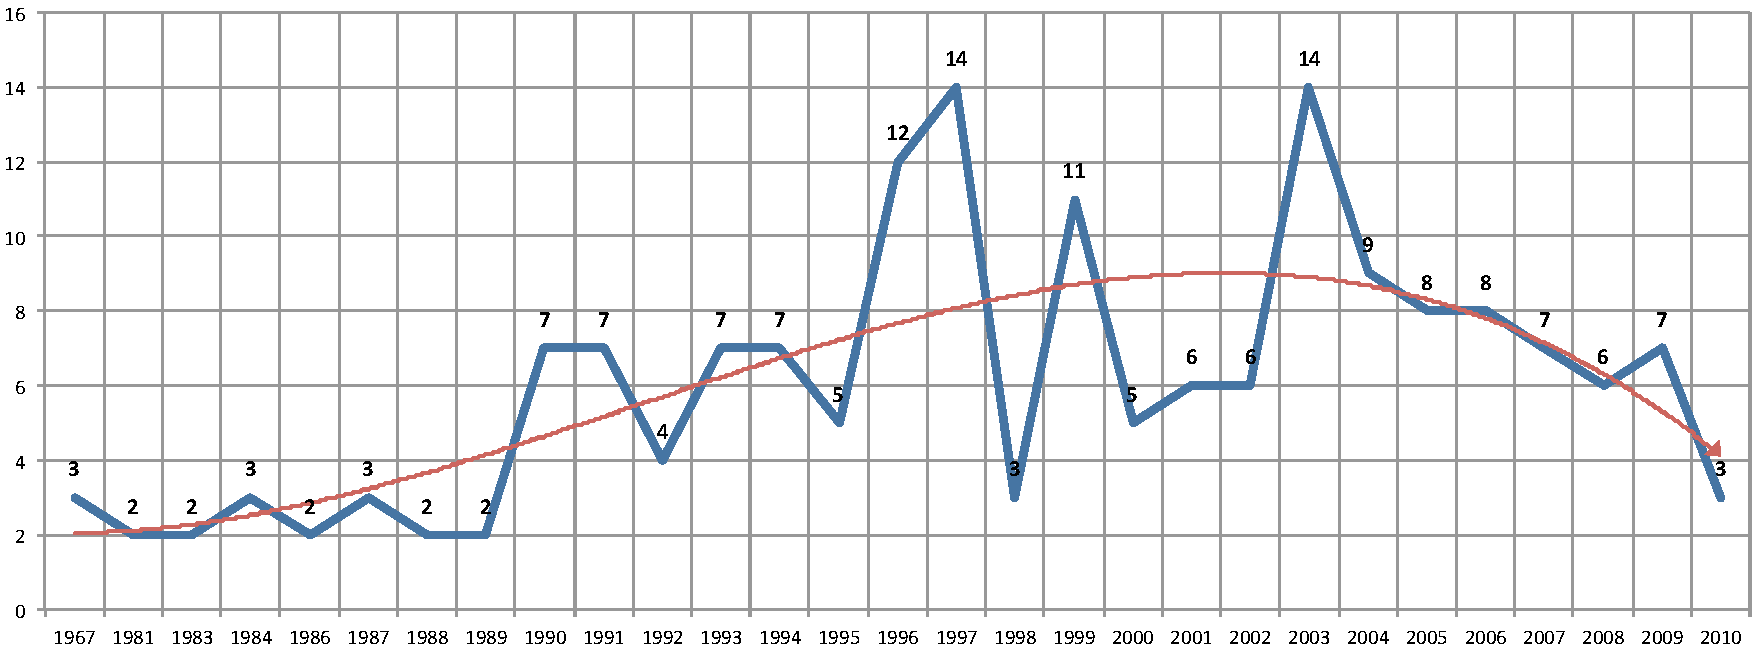
\includegraphics[scale=0.5]{fig/abntex2-modelo-img-grafico.pdf}
	\end{center}
	\legend{Fonte: \cite[p. 24]{araujo2012}}
\end{figure}
\end{verbatim}

Ressalta-se que ao invés de estabelecer a escala da figura através do comando \verb+scale=0.5+, poderia-se definir sua largura ou
altura através de \verb+width+ ou \verb+height+ usando, por exemplo, \\
\verb+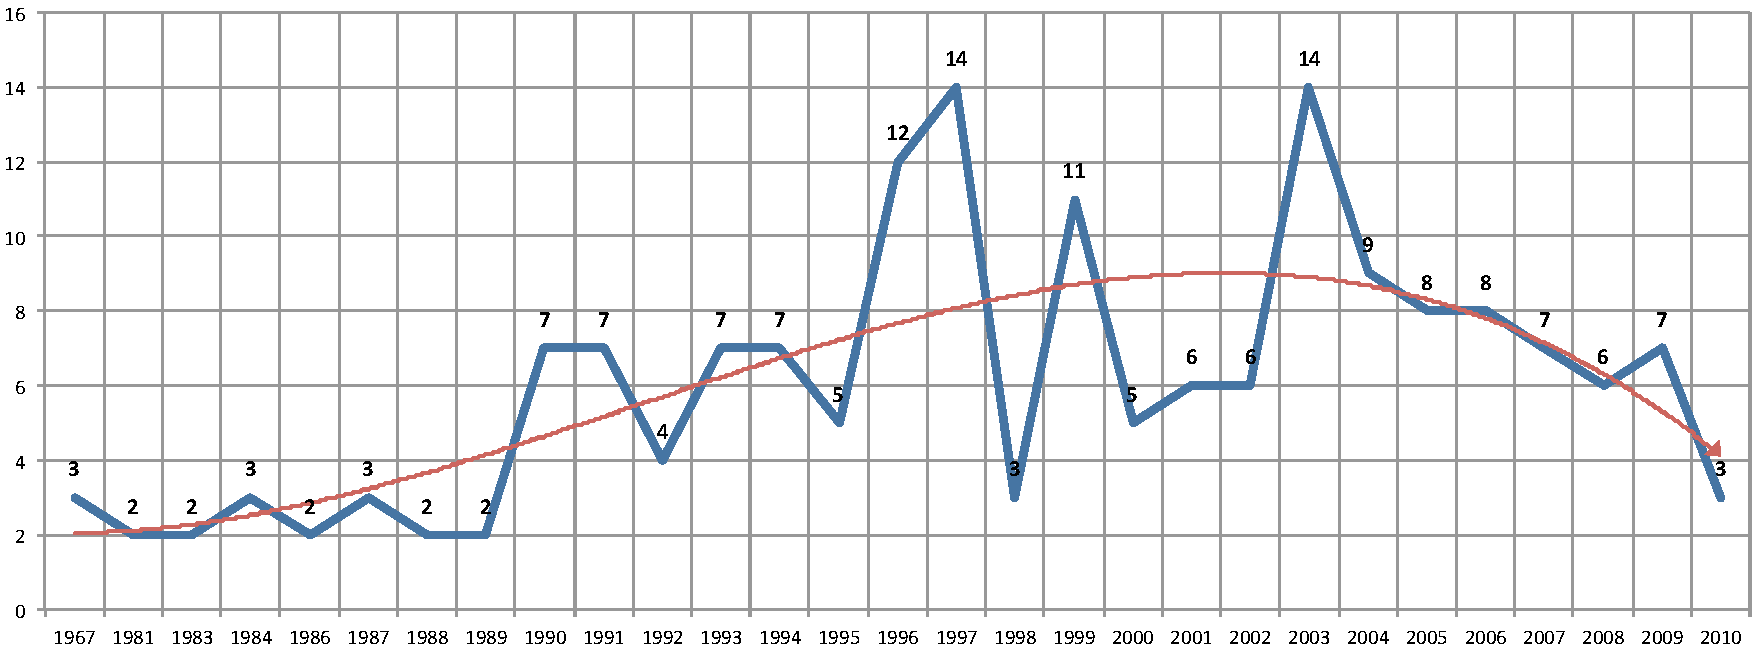
\includegraphics[width=5cm]{fig/abntex2-modelo-img-grafico.pdf}+ que re-escalaria a figura de forma a ela ficar com 5 cm de
largura. Pode-se ainda usar \verb+0.5\linewidth+ ao invés de \verb+5cm+ para estabelecer a largura da figura como sendo metade da
largura da linha do texto. O posicionamento da figura é definido pelo próprio \LaTeX. Recomenda-se colocar o comando o mais próximo
possível do lugar onde a figura é citada. Por fim, recomenda-se usar figuras em formato \verb+pdf+.

\begin{figure}[htb]
	\caption{\label{fig_grafico}Gráfico produzido em Excel e salvo como PDF}
	\begin{center}
	    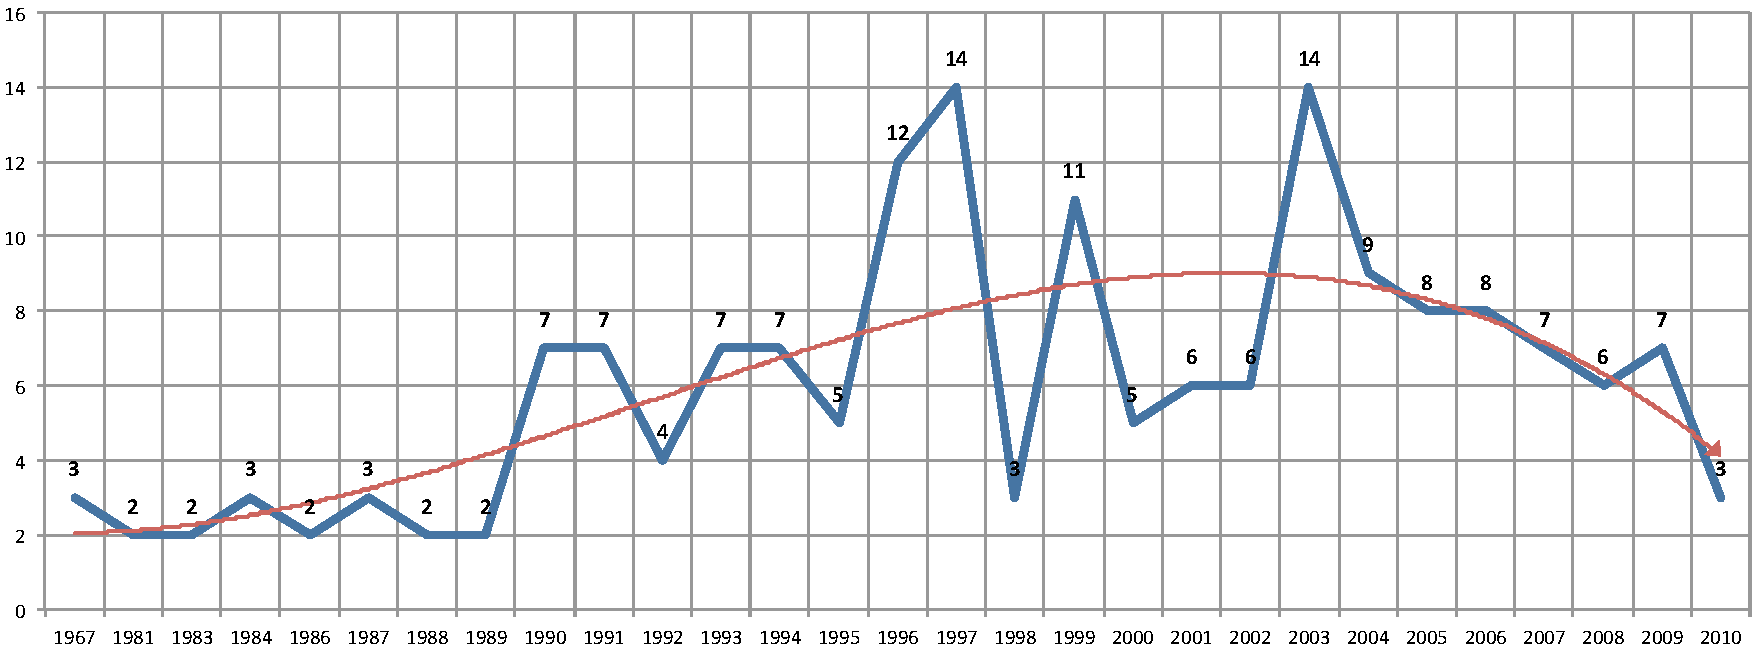
\includegraphics[scale=0.5]{fig/abntex2-modelo-img-grafico.pdf}
	\end{center}
	\legend{Fonte: \cite[p. 24]{araujo2012}}
\end{figure}


\subsection{Tabelas}

Há de se admitir que a confecção de tabelas em \LaTeX\ envolve uma prática um pouco maior. Abaixo apresentamos o comando que gerou a
Tabela~\ref{tab1}. Uma dica interessante é que o comando \verb+\resizebox+ permite ajustar a tabela à largura do texto e é
especialmente útil em situações onde a largura da tabela seria maior que a largura do texto.
\begin{scriptsize}
\begin{verbatim}
\begin{table}[ht] 
    \caption{Publicações relacionadas a alguma área em periódicos selecionados.
    \label{tab1}}
		\resizebox{\linewidth}{!}{%
\begin{tabular}{|l|c|c|c|c|c|c|c|c|c|}
    \hline
\multirow{2}{*}{\textbf{PERIÓDICO}} & \multicolumn{9}{c|}{ANOS}
\\ \cline{2-10}
& 2009&	2010&	2011&	2012&	2013&	2014&	2015& 2016& 2017\\ \hline
\textit{International Journal of Something} &	13&	15&	16&	15&	17&	17&	22& 22& 14\\ \hline 
\textit{Text Horizons}               		& 	6&	6&	9&	6&	8&	7&	19& 7& 6\\ \hline 
\textit{The Blablabla Review}             & 	8&	14&	9&	9&	15&	13&	21& 15& 9\\ \hline 
\textit{Journal of Magic}		&	2&	4&	2&	5&	1&	5&	1& 7& 4\\ \hline 
\textbf{TOTAL}&                           	29&	39&	36&	35&	41&	42&	63& 51& 33\\ \hline 
\multicolumn{8}{l}{Confeccionado pelo autor.}
\end{tabular}%
}
\end{table}
\end{verbatim}
\end{scriptsize}

\begin{table}[ht] 
    \caption{Publicações relacionadas a alguma área em periódicos selecionados.
    \label{tab1}}
		\resizebox{\linewidth}{!}{%
\begin{tabular}{|l|c|c|c|c|c|c|c|c|c|}
    \hline
\multirow{2}{*}{\textbf{PERIÓDICO}} & \multicolumn{9}{c|}{ANOS}
\\ \cline{2-10}
& 2009&	2010&	2011&	2012&	2013&	2014&	2015& 2016& 2017\\ \hline
\textit{International Journal of Something} &	13&	15&	16&	15&	17&	17&	22& 22& 14\\ \hline 
\textit{Text Horizons}               		& 	6&	6&	9&	6&	8&	7&	19& 7& 6\\ \hline 
\textit{The Blablabla Review}             & 	8&	14&	9&	9&	15&	13&	21& 15& 9\\ \hline 
\textit{Journal of Magic}		&	2&	4&	2&	5&	1&	5&	1& 7& 4\\ \hline 
\textbf{TOTAL}&                           	29&	39&	36&	35&	41&	42&	63& 51& 33\\ \hline 
\multicolumn{8}{l}{Confeccionado pelo autor.}
\end{tabular}%
}
\end{table}


\chapter{Conclusions}

Conclusões.


\chapter{Introduction}

In 1951 the Belousov-Zhabotinsky class of chemical reactions were created for the first time in a laboratory. They would become a
classic example of non-equilibrium thermodynamics and helped instigate interest in the sub-area of complex systems: coupled
oscillators. In the decades that followed other areas of research led, independently, to the same interest in studying coupled
oscillators systems. In 1958, Norbet Weiner at the MIT was looking at power spectrum graphs generated from brain scans and decided that
there must be some kind of synchronization amongst many coupled, periodically-firing, neurons. Also inspired by the many biological
rhythms observed in nature, Arthur Winfree published in 1967 a paper on the mathematical modelling of interacting oscillators. Winfree
defined a phase oscillator as an abstraction of a system that possesses a closed loop in its phase-space. A single real number between
$0$ and $2\pi$ could describe, for example, a living cell that undergoes any kind of periodic cycle. The major simplification comes
from the fact that when two such phase oscillators interact, each influences {\textit only} the phase value of the other. Their
trajectories in phase space are assumed to be fixed, and only the velocity with which they traverse it is influenced by the coupling.

Seven years after Winfree's paper from 1967, the then young Japanese scientist Yoshiki Kuramoto was inspired by it. He recognized what
made Winfree's model hard to solve and proposed an arguably less realistic version of it, but the beauty of the now possible
mathematical solution made up for it. So much so that it got it's own name, the Kuramoto model, one of the major founding stones of
modern investigations on these kinds of dynamical systems.

This work could be considered as one such branch, where the phase value that describes a unit has been discretized into only three
possible values, $0$, $2\pi/3$ and $4\pi/3$. These types of discrete phase models saw much use in describing systems which present
distinct states. One such system is interacting neurons, where one could choose to represent three different neuronal states as firing
($\varphi_0$), refractory ($\varphi_1$) and ready-to-fire ($\varphi_2$). Another phenomenon explained by one such model is the
synchronous blinking of some firefly species, which had long been reported but scientists were skeptical of it until camera recorders
got around. If $n$ state representations are desired than the phase value of each unit would be one of $\{\varphi_0 ...
\varphi_{n-1}\}$ with $\varphi_{n}=\varphi_0$.
% TODO: Why was stochasticity introduced to these models?


\chapter{Kuramoto Model}


In this chapter we describe the Kuramoto model and reproduce his self-consistency arguments that allow for a synchronous phase to
emerge at some critical coupling. In order to do this an order parameter must be introduced together with a mean-field approximation.
The stability analysis of the solutions of the Kuramoto model took decades to develop and led to some very anti-intuitive findings such
as the fact that the disordered phase for low-couplings is not stable, but neutrally stable, and is related to Landau damping in plasma
physics. These later discussions are not in the scope of this chapter.

\section{Equation}

The Kuramoto model deals with an infinite number of phase oscillators which are all coupled to each other. We start with a collection
of $N$ oscillators and then take the limit $N \to \infty$. Each unit is described by its phase value $\varphi_i$ and its natural
frequency $\omega_i$. The natural frequency is the frequency with which an isolated oscillator rotates. The population of oscillators
are assumed to have some distribution $g(\omega)$ which is symmetric about some frequency $\omega_0$ and has a single maximum at this
same value.

The biologically inspired Winfree model states that at every instant, each oscillator sends a signal of strength $P(\varphi)$ and
responds by adjusting its own phase value by an amount $R(\varphi)$, which is captured in the equation:

\begin{equation}
    \label{winfreeeq}
    \dot{\varphi_j} = \omega_j + \frac{1}{N}\sum_{k=1}^{N}P(\varphi_k)R(\varphi_j), \qquad i=1,...,N
\end{equation}

To make this solvable, we say that the angular frequency of a unit depends only on its relative phase to others. Furthermore, this
dependency is through a sine kernel. This will make possible the self consistency arguments done later. This set of assumptions
transforms (\ref{winfreeeq}) into:

\begin{equation}
    \label{kuramotoeq}
    \dot{\varphi_j} = \omega_j + \frac{K}{N}\sum_{k=1}^{N}sin(\varphi_k - \varphi_j), \qquad i=1,...,N
\end{equation}

\noindent where $K>0$ is a real constant which describes the coupling strength and  $N>>1$.

\section{Order Parameter}

\section{Fubar}

\subsection{Fufoobar}

Fubbar

\subsection{Fubfoo}

f... BAR!

\subsection{F}

.

\chapter{Fooblusions}

b




% ----------------------------------------------------------
% ELEMENTOS PÓS-TEXTUAIS
% ----------------------------------------------------------
\postextual
% ----------------------------------------------------------

% ----------------------------------------------------------
% Referências bibliográficas
% ----------------------------------------------------------
\bibliographystyle{babunsrt}
\bibliography{tex/references}

% ----------------------------------------------------------
% Glossário
% ----------------------------------------------------------
%
% Consulte o manual da classe abntex2 para orientações sobre o glossário.
%
%\glossary

% ----------------------------------------------------------
% Apêndices
% ----------------------------------------------------------

% ---
% Inicia os apêndices
% ---
\begin{apendicesenv}

% Imprime uma página indicando o início dos apêndices
\partapendices

% ----------------------------------------------------------
\chapter{\label{appendix:LC}Path length and clustering for regular ring lattices}
% ----------------------------------------------------------

\section{Average Path Length}

The distance $L_{ij}$ between two nodes $i$ and $j$ is the minimum number of edges that must be traversed to connect them. The average
path length is defined as the average distance between every possible pair of nodes in the network. For a network with $N$ nodes this
is:

\begin{equation}
    L = \frac{2}{N^2-N}\sum_{i<j}L_{ij}
\end{equation}

Consider the lowest node in a ring graph with $N$ nodes and $2K$ neighbors per node. Going counterclockwise (CCW), there are $K$ nodes
at distance $1$, then $K$ nodes at distance $2$ and so on until we reach some region near the top. In total, there will be $G$ groups
of nodes, each with $K$ nodes, at distances $1,2,3...,G$ from our starting point at the bottom. $G$ is given by the largest integer
smaller than $(N-1)/(2K)$. This can be written with the floor operation:

\begin{equation}
    G=\floor*{\frac{N-1}{2K}}
\end{equation}

This same procedure can be performed from the clockwise (CW) direction. Thus, there are $2K$ nodes at distance $1$ and so on up to
distance $G$. The last group of nodes at the top is therefore at a distance $G+1$, but it contains less than $2K$ nodes. Indeed, it
contains a number $R$ of nodes equal to the remainder of the integer division of $N-1$ by $2K$:

\begin{equation}
    R = N - 1 - 2KG
    \label{eq:R}
\end{equation}

\noindent This reasoning can be visualized in Fig.~\ref{fig:Lgroups}.

\begin{figure}
\centering
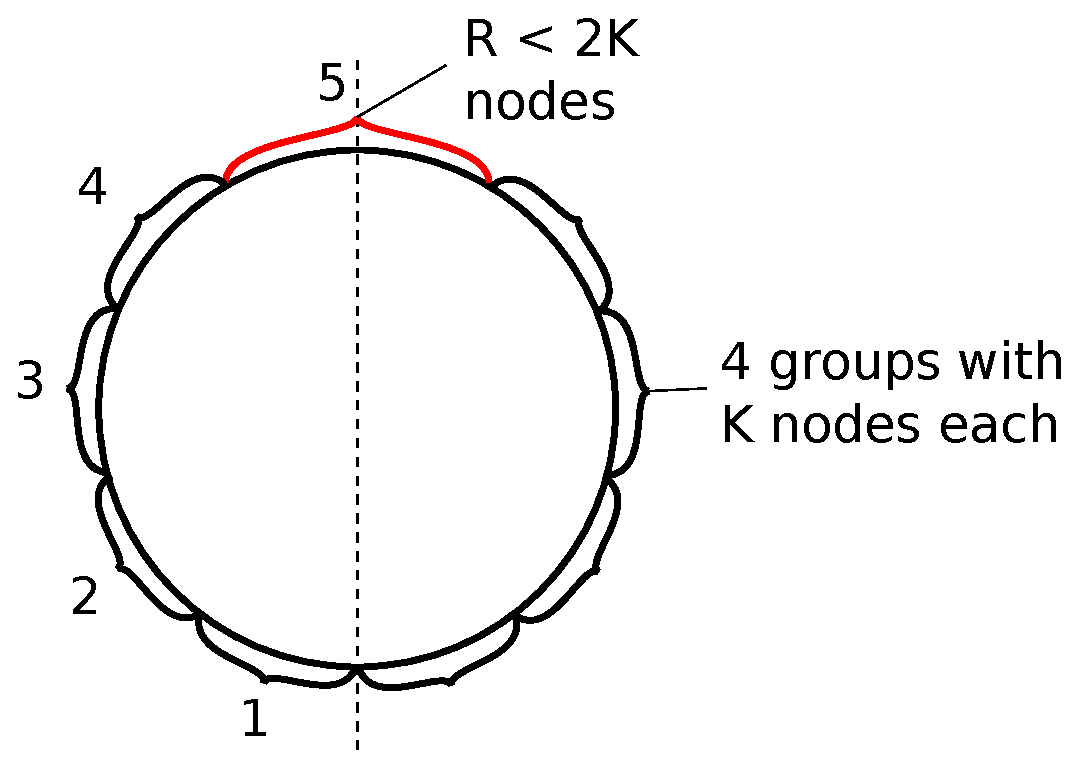
\includegraphics[width=0.6\textwidth]{fig/path_length_groups.eps}
\caption{Counting the number of nodes at distances visually. Here $G=4$ groups at distances $1,2,3,4$ from the bottom node.}
\label{fig:Lgroups}
\end{figure}

Since there are $N-1$ pairs between the bottom node and all other nodes in the lattice, the average distance $L_0$ between the bottom
node and all other nodes is then given by:

\begin{align}
    L_0 &= \frac{1}{N-1} \left[ 2K \sum_{i=1}^Gi + R(G+1) \right] \notag \\[9pt]
        &= \frac{1}{N-1} \left[ KG(G+1) + R(G+1) \right] \notag \\[9pt]
    L_0 &= \left(G + 1\right) \left( 1 - \frac{KG}{N-1} \right)
\end{align}

\noindent where we used equation \ref{eq:R} to substitute in for $R$.  Because we started with an arbitrary node at the bottom, this
result is true for any given node in a regular ring, and thus we conclude that the average path length for the whole network is just
$L_0$.

\begin{align}
    L(N,K) = \left(G + 1\right) \left( 1 - \frac{KG}{N-1} \right) \notag \\[9pt]
    \text{with} \qquad G=\floor*{\frac{N-1}{2K}}
\end{align}

\section{Average Clustering}

The clustering coefficient for a node $i$ in the graph is defined as: let $n_i$ be the number of neighbors of some node $i$. Then,
there are at most $(n_i^2-n_i)/2$ connections between any two of its neighbors. Let $m_i$ be the number of actual connections that are
present in a particular graph. Then, the clustering coefficient $C_i$ of node $i$ is given by:

\begin{equation}
    C_i = \frac{2m_i}{n_i^2-n_i}
\end{equation}

\noindent If there are $N$ nodes in the graph, the average clustering
coefficient is thus given by:

\begin{equation}
    C = \frac{1}{N}\sum^N_{i=1} C_i
\end{equation}

First, consider a ``close-up" of a section of a regular ring where $N\gg K$.  Consider a node $i$ with $K$ CW neighbors and $K$ CCW
neighbors. Let $m$ be the number of connections between neighbors of node $i$. We can manually count $m$ for some values of $K$:

\begin{figure}
\centering
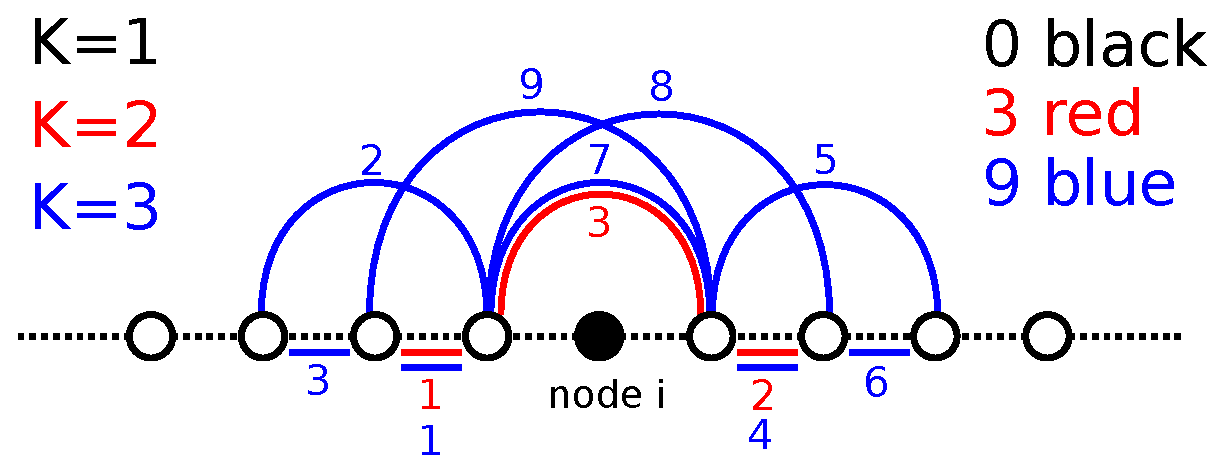
\includegraphics[width=0.75\textwidth]{fig/clustering.eps}
\caption{ (Color online) Counting $m$ for $k=1,2,3$. We note three contributions to $m$: a fully connected group of $K$ CW neighbors
(left), a fully connected group of $K$ CCW neighbors (right) and connections that go ``over" the center node.  }
\label{fig:clustering}
\end{figure}

\begin{align*}
    m &= 0 \qquad \text{if} \qquad K \leq 1\\
    m &= 3 \qquad \text{if} \qquad K = 2\\
    m &= 9 \qquad \text{if} \qquad K = 3
\end{align*}

The general case for $N \gg K$ can be counted by summing the contributions of the three groups as shown in figure \ref{fig:clustering}.
Two fully connected groups of $K$ nodes each contributes with $(K^2-K)$ connections. The connections that bypass node $i$ also
contribute with $(K^2-K)/2$ connections and thus we have.

\begin{align}
    m &= \frac{3}{2}(K^2-K)
    \label{eq:m}
\end{align}

\noindent Now we divide equation \ref{eq:m} by the total number of connections between the $2K$ neighbors of node $i$ to get its
clustering coefficient $C_i$:

\begin{align}
    C_i(N,K) = \frac{3K-3}{4K-2}
    \label{eq:ci}
\end{align}


\begin{figure}
\centering
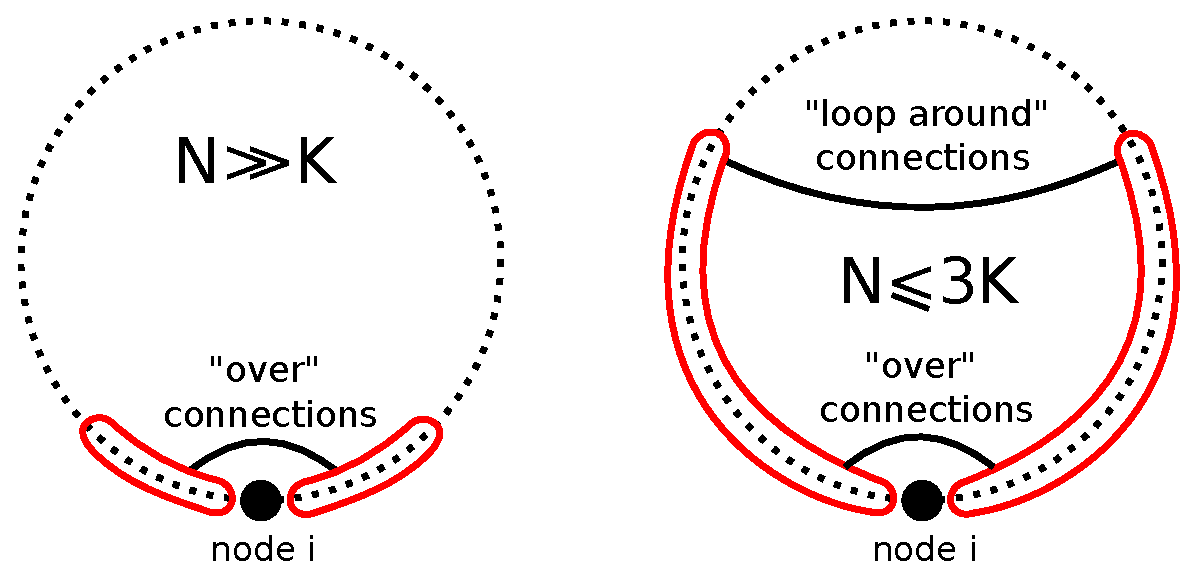
\includegraphics[width=0.9\textwidth]{fig/clustering-loop.eps}
\caption{ Connections that contribute to the clustering coefficient of node $i$.  The red regions represent the CW and CCW groups of
neighbors of node $i$, and they are fully connected each within itself. Additional connections are made going ``over" node $i$, but
when $N\leq3K$ there are additional connections that loop around the opposite side of the lattice.  }
\label{fig:loop}
\end{figure}

\noindent When $N$ is not so large compared to $K$, additional connections between the CCW and CW neighbors may appear by looping
around the opposite side of node $i$, as depicted in figure \ref{fig:loop}. These additional connections will be present whenever the
remaining nodes that are neither in the CW or CCW group are fewer than $K$. The number of such nodes is just $N-2K-1$, which gives us
the condition $N\leq 3K$ for additional connections to be present.


The number of ``loop around" connections that will be present will depend on how many nodes there are in the remaining group after
removing node $i$ and its immediate neighbors. Let this number be denoted by $D=N-2K-1$. Then, the number of additional connections
will be given by

\begin{align}
    (K-D) + (K-D-1) + ... + 2 + 1 = \frac{(K-D+1)(K-D)}{2}
    \label{eq:looparound}
\end{align}

Adding equation \ref{eq:looparound} to \ref{eq:m} we get

\begin{align}
    m = \frac{3}{2}(K^2 - K) + \frac{1}{2}(3K-N+1)(3K-N+2)
\end{align}

And thus the clustering now becomes:

\begin{align}
    C_i(N,K) = \frac{3K-3}{4K-2} + \frac{(3K-N+1)(3K-N+2)}{4K^2-2K}
    \label{eq:ci1}
\end{align}

This formula holds up to the point when $D=0$ or $N=2K+1$. For all values $D\leq 0$ the regular ring is in fact a complete graph, where
every node connects to every other. In these cases the clustering coefficient is always equal to one.  Formulas \ref{eq:ci} and
\ref{eq:ci1} together offer a complete expression for the clustering of node $i$. Since $C_i=C_j \quad \forall i,j$, this is just the
average clustering of the whole network and we finally get:

\begin{align}
    C(N,K) =
    \begin{cases}
        \frac{3K-3}{4K-2} \quad &\text{if} \quad N>3K \\[9pt]
        \frac{3K-3}{4K-2} + \frac{(3K-N+1)(3K-N+2)}{4K^2-2K} \quad &\text{if}
        \quad 3K \geq N > 2K+1 \\[9pt]
        1 \quad &\text{else}
    \end{cases}
    \label{eq:ci2}
\end{align}


\end{apendicesenv}


% ----------------------------------------------------------
% Annex
% ----------------------------------------------------------
%\begin{anexosenv}
%
%
%\partanexos  % Print annex front page
%
%\chapter{My annex 1}
%\chapter{My annex 2}
%
%
%\end{anexosenv}

%---------------------------------------------------------------------
% INDICE REMISSIVO - ELEMENTO OPCIONAL
%---------------------------------------------------------------------
%\phantompart
%\printindex
%---------------------------------------------------------------------


\end{document}
